% Created 2019-09-21 Sat 22:27
% Intended LaTeX compiler: pdflatex
\documentclass[presentation]{beamer}
\usepackage[utf8]{inputenc}
\usepackage[T1]{fontenc}
\usepackage{graphicx}
\usepackage{grffile}
\usepackage{longtable}
\usepackage{wrapfig}
\usepackage{rotating}
\usepackage[normalem]{ulem}
\usepackage{amsmath}
\usepackage{textcomp}
\usepackage{amssymb}
\usepackage{capt-of}
\usepackage{hyperref}
\usepackage{minted}
\setminted{fontsize=\scriptsize,baselinestretch=1}
\usemintedstyle{monokai}
\usetheme{metropolis}
\author{Igor Dejanović\textsuperscript{1}, Mirjana Dejanović\textsuperscript{2}}
\date{September, 2019 @ ERK Portorož Slovenia}
\title{Generating program code for psychological experiments from high-level descriptions}
\subtitle{University of Novi Sad\textsuperscript{1}, University of Priština\textsuperscript{2}}
\hypersetup{
 pdfauthor={Igor Dejanović\textsuperscript{1}, Mirjana Dejanović\textsuperscript{2}},
 pdftitle={Generating program code for psychological experiments from high-level descriptions},
 pdfkeywords={},
 pdfsubject={},
 pdfcreator={Emacs 26.3 (Org mode 9.2.6)}, 
 pdflang={English}}
\begin{document}

\maketitle

\section*{Introduction}
\label{sec:orgead1246}
\begin{frame}[label={sec:orgc5c63ec}]{Experimental Psychology}
\end{frame}

\begin{frame}[label={sec:orgf695c52}]{An example -- the Simon effect test}
\begin{center}
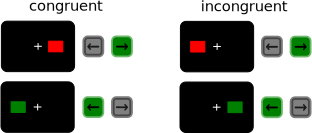
\includegraphics[width=1\textwidth]{./images/simon_experiment.png}
\end{center} 
\end{frame}
\begin{frame}[label={sec:orgdf95a49}]{}
\begin{center}\huge{Motivation}\end{center}
\end{frame}

\section*{Domain-Specific Languages}
\label{sec:orgc3b4fe4}
\begin{frame}[label={sec:org6205fe3}]{What are they?}
\end{frame}

\begin{frame}[label={sec:org101c989}]{}
\vfill
\begin{center}
\includegraphics[width=.9\linewidth]{./images/textX.png}
\end{center} 
\begin{center}
\fontsize{9pt}\selectfont
\url{https://github.com/textX/textX}
\end{center}
\fontsize{6pt}\selectfont
\begin{quote}
I. Dejanović, R. Vaderna, G. Milosavljević, Ž. Vuković, TextX: A Python tool for
Domain-Specific Languages implementation, Knowledge-Based Systems 115,
1-4, 2017.
\end{quote}
\end{frame}
\section*{pyFlies}
\label{sec:org0e86e33}
\begin{frame}[label={sec:org881de09},fragile]{pyFlies code for the Simon effect test}
 \begin{minted}[]{text}
test Simon {
  conditions {
    position  color  congruency   response

    left      green  congruent    left
    left      red    incongruent  right
    right     green  incongruent  left
    right     red    congruent    right
  }

  stimuli{
    all: shape(rectangle, position position,
               color color)
    error: sound(1000)
    fixation: shape(cross)
  }
}
\end{minted}
\end{frame}

\begin{frame}[label={sec:orgf20c55c}]{Target code generators}
\begin{center}
\includegraphics[width=1\textwidth]{./images/architecture.png}
\end{center} 
\end{frame}

\begin{frame}[label={sec:orgc5af548}]{Template engines}
\begin{center}
\includegraphics[width=1\textwidth]{./images/template_engine.png}
\end{center} 
\end{frame}

\section*{Conclusion}
\label{sec:org3ec729e}
\section*{Thanks! Q\&A?}
\label{sec:orgbee0eb6}
\end{document}